% \documentclass[10pt,a4paper]{article}
% \include{header}
% \appendtographicspath{{/home/debortoli/research/patch_sim/res_percep/}{/home/debortoli/research/patch_sim/res/}{./eps2pdf/}}
% \bibliography{/home/debortoli/research/research.bib}
% \title{Patch similarity} \author{Valentin De Bortoli}
% \begin{document}
In our study $X$ will be a stochastic process defined on $\Omega$ where
$\Omega = \left(\mathbb{Z} \backslash M\mathbb{Z} \right) \times \left(
  \mathbb{Z} \backslash N\mathbb{Z} \right) := \mathbb{T}_M \times
\mathbb{T}_N$, or $\Omega = \mathbb{T}^2$, or $\Omega = \mathbb{Z}^2$ or
$\Omega = \mathbb{R}^2$. Let $\mathcal{P}$ a subset of $\Omega$, $\mathcal{P}$
will be called patch indices and $X(\mathcal{P})$, respectively
$X_0(\mathcal{P})$, are called patches in $X$, respectively in
$X_0$. $s(\cdot,\cdot)$ will denote a patch similarity function.  Details about
this function will be introduced in the next section. For $t \in \Omega$ we
introduce the shift operator $\tau_t$.
\section{Patch similarity functions}
The different possibilities for $\Omega$ will be studied in this document. $X_0$ will be a
template image also defined on $\Omega$.  Both $X_0$ and $X$ take their values
in $\mathbb{R}$.  In this section we investigate patch similarity function.  Our
goal is to find a similarity function which is tractable with an \acontrario \
setting and presents good visual properties. To our knowledge there exists no
review on the subject. We are looking for similarity functions which do not use
a probabilistic background since this background will be introduced using an
\acontrario \ model. In \cite{deledalle2012compare} the authors present similarity functions but most
of them are based on a frequentist or bayesian approach thus not appropriate in
our setting. Some popular patch similarity functions are based on modified euclidean distances, $i.e$ positive definite quadratic forms. This approach was used in denoising applications \cite{buades2005non}. In \cite{delon2013patch}, the authors derived optimal weights to discriminate identical patches. \\
\comment{ (10/10) j'ai posé la question à Sivic qui, en cours d'object
  recognition, parle de norme euclidienne entre des patches. A sa connaissance à
  part la cross-correlation il n'y a pas d'autres normes typiques utilisées (du
  moins qui lui venait directement à l'esprit lorsque je lui ai posé la
  question). Néanmoins il m'a dit (et j'ai pu constater en faisant une petite
  recherche bibliographique) que de nouvelles fonctions de similarité étaient
  déterminées \textit{via} du learning. Peut-être que ces fonctions pourraient
  être calculées dans un premier temps puis utilisées dans le cadre \acontrario
  . Faut-il évoquer d'autres mesures plus empiriques comme SSIM ?} These patch similarity functions will be used in two different settings:
\begin{itemize}
\item \textit{internal matching:}
  $s\left(X(\mathcal{P}), \tau_t(X)(\mathcal{P})\right)$ measures the similarity
  between a patch in $X$ and its shifted version in $X$.  In an \acontrario \
  setting an offset $t$ will be detected if a patch and its shifted version
  present a similarity which is not likely to be present in the background
  stochastic model.  This can be used in periodicity analysis or in a
  variational context.
\item \textit{template matching:}
  $s\left(X_0(\mathcal{P}), \tau_t(X)(\mathcal{P}) \right)$ measures the
  similarity between a patch template and the patches in $X$. In an \acontrario \
  setting \ $X$ can be generated as a textured version of
  $X_0(\mathcal{P})$. This similarity function can be used in a discriminative,
  or parametric, texture synthesis algorithm.  The terminology \textit{template
    matching} was introduced in \cite{deledalle2012compare}.
\end{itemize}
Now we want to investigate patch similarity functions which are tractable in the
sense that either $s\left(X(\mathcal{P}), \tau_t(X)(\mathcal{P})\right)$ or
$s\left(X_0(\mathcal{P}), \tau_t(X)(\mathcal{P})\right)$ probability density
functions can be computed. We need to precise the underlying stochastic process
$X$. Usually $X$ will be a white noise, a \DSN \ model or an \ADSN \ model.\\
\comment{(10/10) d'autres modèles à voir ?  } Tractability issues occur only
considering discretizations of our setting. Thus we will not bother considering
these issues in the continuous domain.  However it will still be of interest to
derive properties in the continuous domain. Table \ref{tab:patch_sim} gives a brief summary of
the similarity functions studied in this report and their properties.
% EN LIGNES LES DIFFERENTES DISTANCES QUI PEUVENT ETRES UTILISÉES PDF ?
% PROPERTIES
\begin{table}[h]
  \begin{tabularx}{\textwidth}{|c||X|X|}
    \hline
    Patch similarity function & Internal matching & Template matching \\ \hline \hline
    $s_{\|\cdot\|,2}(A,B) = \| A-B \|_2$ & non-asymptotic expression  &  non-asymptotic expression \\ \hline
    $s_{\langle \cdot\rangle,2}(A,B) = \langle A,B \rangle$ & asymptotic expression, Gaussian  &  asymptotic expression, Gaussian \\ \hline
    $s_{\cos,2}(A,B) = \frac{\langle A,B \rangle}{\|A\|_2\|B\|_2}$ &  asymptotic expression, Gaussian &   asymptotic expression, Gaussian \\ \hline
    $s_{\|\cdot\|,1}(A,B) = \| A-B \|_1$ & not tractable  &  not tractable \\ \hline
    $s_{\|\cdot\|,\infty}(A,B) = \| A-B \|_{\infty}$ & not tractable  &  not tractable \\ \hline    
  \end{tabularx}
  \caption{A summary of the properties of the different patch similarity functions investigated}
  \label{tab:patch_sim}
\end{table}
\subparagraph{Features} We compute the patch similarity functions quantity
directly on patch pixel values. It can be interesting to compute features on the
images and then make use of the patch similarity function.  For example in \cite{patraucean2013detection} the authors compute the gradient of the original image. The model image is a
white noise and thus looking at the orientation of its gradient we obtain an
uniform probability density function. To be precise if the gradient is computed
using finite differences the gradient is computed in the model image on a
thinner grid (or is computed exactly in a continuous setting), otherwise the
gradient orientations are not independent. Linear filtering is another
option. One could note that in a centered Gaussian case this simply amounts to
changing the covariance function.  \subparagraph{} In the following subsection
we give details about the results stated in Table \ref{tab:patch_sim}. For every similarity
function we try to give results for the different probabilistic settings and
$\Omega$ sets.
\subsection {\acontrario \ setting}
We restrict ourselves to $\Omega_{N,M} := \mathbb{T}_m \times \mathbb{T}_N$, the set of definition of discrete periodic images. For
implementation purposes this framework will be chosen. However the periodic
assumption is not always satisfied. Several solutions exist to project periodic
functions onto the set of the periodic functions \cite{moisan2011periodic}, however they all suffer
from drawbacks. This problem will not be addressed here.  \subsubsection{\s2
  patch similarity function} We will not study \s2 directly but
$s_2 = s_{\| \cdot \|, 2} ^2$. Before stating a few results let us introduce some
notions.
\begin{mydef}[Autocorrelation]
  Let $h$ defined on $\Omega$. We define the autocorrelation $A_h$ on $\Omega$,
  \[A_h = \frac{1}{MN} h * \check{h} \] Note that $A_h$ takes real values and is
  symmetric.
\end{mydef}
\comment{
  (19/10)
  En fait il faut introduire l'autocorrélation dans le cadre général des modèles ADSN définis comme limite de modèle de fermés stochastiques. Faire le lien entre le modèle sur une grille discrète et sur une grille périodique. Remarquer notamment que l'on n'a pas de corrélation à longue distance à prendre en compte (ce qui rendait le thm faux).}
Let us focus on the \internalmatching . We derive the following property.
\begin{prop}
  Let $X$ be a Gaussian field on $\Omega$ with mean $0$ and covariance matrix
  $C$, then
  \[s_2\left(X(\mathcal{P}), \tau_t(X)(\mathcal{P})\right) \sim \summ{x \in
      \mathcal{P}}{}{\lambda_x \xi_x}\] where $(\xi_x)_{x \in \mathcal{P}}$ are
  independent chi-square variables with one degree of freedom and
  $(\lambda_x)_{x \in \mathcal{P}}$ are the eigenvalues of
  $\Gamma_{\mathcal{P}} \in \mathcal{M}_{\vert \mathcal{P} \vert}\left(
    \mathbb{R} \right)$, with
  \[ \Gamma_{\mathcal{P}}(x,x') = C(x, x') + C(t+x, t+x') - C(x,t+x') -
    C(x+t,x').
  \]
\end{prop}
We must distinguish two cases:
\begin{itemize}
\item white noise case $C(x,x') = \delta_{x,x'}$ and
  $\Gamma_{\mathcal{P}} = 2\delta_{x,x'} - \delta_{x,x'+t} - \delta_{x,x'-t}$,
\item \ADSN \ case where $C(x,x') = A_h(x-x')$ ($h$ is a function defined on
  $\Omega$) and
  \[\Gamma_{\mathcal{P}} = 2A_h(x-x') - A_h(x-x'-t) - A_h(x-x'+t) .\]
\end{itemize}
In both cases $\Gamma_{\mathcal{P}}$ is block symmetric with symmetric blocks, positive semi-definite and Toeplitz with Toeplitz blocks. Eigenvalues can be computed using a block circulant with circulant blocks approximation and in the white noise case closed forms can be derived for the eigenvalues. Another problem is sampling a weighted sum of independent chi-square variables. A large literature exists on the subject \cite{wood1989f}, \cite{moschopoulos1984distribution}, \cite{box1954some}, \cite{imhof1961computing}, \cite{jensen1972gaussian}, \cite{kotz1967series}, \cite{bodenham2016comparison}.\\
Now we present results in \templatematching .
\begin{prop}
  Let $X$ be a Gaussian field on $\Omega$ with mean $0$ and covariance matrix
  $C$, then
  \[s_2\left(X_0(\mathcal{P}), \tau_t(X)(\mathcal{P}) \right) \sim \summ{x \in
      \Omega}{}{\lambda_x}{\tilde{\xi}_x}\] where
  $\left( \tilde{\xi}_x\right)_{x\in \mathcal{P}}$ are independent non centered
  chi-square variables with one degree of freedom and non centering parameter
  $\left(-P_t X_0(\mathcal{P}) (x) \right)_{x \in \mathcal{P}}$ where
  $P_t \in \mathcal{O}_{\vert \mathcal{P} \vert}\left( \mathbb{R} \right)$ such
  that $P_t D P_t^T = C_{\tau_{-t}\left(\mathcal{P}\right)}$
  ($C_{\tau_{-t}\left(\mathcal{P}\right)}$ is the restriction of $C$ to the
  $\tau_{-t}\left(\mathcal{P}\right)$ indices) and where
  $(\lambda_x)_{x\in\tau_{-t}\left(\mathcal{P}\right)}$ are the eigenvalues of
  $C_{\tau_{-t}\left(\mathcal{P}\right)}$.
\end{prop}
In the special case where $X$ is a white noise, $P_t$ is the identity matrix and ${\forall x \in \mathcal{P}, \lambda_x = 1}$. As before there exists techniques to easily compute approximations of the eigenvalues of the restricted matrices. The main difficulty is to sample from a weighted sum of non centered independent chi-square random variables.\\
\comment{(10/10) je devrais procéder à une bibliographie sur le sujet mais des
  techniques issues du cas centré peuvent être exportées dans le cas non
  centrés, je pense à Imhof notamment.}

\subsubsection{\sps \ patch similarity function} Since template matching is intractable
in the \s2 \ case we only consider the scalar product. The idea of considering scalar product
instead of Euclidean norm can be found in \cite{riot2017correlation}. Concerning the
\internalmatching \ \sps \ seems intractable. Indeed denoting
$p_{\mathcal{P}} \in \mathcal{M}_{\vert \mathcal{P} \vert, \vert \Omega
  \vert}\left( \mathbb{R} \right)$ the projection matrix onto the subspace
spanned by $(X(x))_{x\in \mathcal{P}}$ we obtain that
\[s_{\langle \cdot \rangle, 2}\left(X(\mathcal{P}),
    \tau_t(X)(\mathcal{P})\right) = X^T p_{\mathcal{P}}^T
  p_{\tau_t(\mathcal{P})} X\] Let
$A = p_{\mathcal{P}}^T p_{\tau_t(\mathcal{P})}$. $A$ is not symmetric and we
even have
\[\forall (x,x') \in \Omega^2, \ AA^T(x,x') = , \ \text{and} \ A^TA(x,x')\]
Thus $A$ is not normal and cannot be diagonalized using orthonormal
matrices. Thus \sps \ cannot be written as a weighted sum of chi-square random
variables. This conclusion holds for every Gaussian field with mean $0$. However
asymptotic results can be derived.
\begin{prop}
  Let $X$ be a Gaussian field defined on $\mathbb{Z}^2$. We define
  $\left(X_{M_k,N_k}\right)_{k \in \mathbb{N}}$ a sequence of Gaussian fields
  defined on $\Omega_{M_k,N_k} := \mathbb{T}_{M_k} \times \mathbb{T}_{N_k}$ such
  that $X_{M_k,N_k}(\Omega_{M_k,N_k}) = X(\Omega_{M_k,N_k})$. We suppose $X$ is
  stationary and its covariance matrix is given by
  $\forall (x,x') \in \mathbb{Z}^2, \ C(x,x') = R_X(\vertt{x-x'}) =
  A_h(x-x')$. We also suppose that $h$ has compact support. Let
  $\seq{\mathcal{P}}{k}$ be a sequence of increasing sets such that
  $\mathcal{P}_k \in \Omega_{M_k,N_k}$ then we have
  \[\vertt{\mathcal{P}_k}^{-1} s_{\langle \cdot
      \rangle,2}\left(X_{M_k,N_k}(\mathcal{P}_k),
      X_{M_k,N_k}(\tau_t(X_{M_k,N_k})(\mathcal{P}_k) \right) \ \underset{k
      \rightarrow +\infty}{\overset{\text{a.s}}{\longrightarrow}} A_h(t).\]
\end{prop}
\remark{Note that for $k$ large enough $X_{M_k,N_k}$ has the same p.d.f as an
  \ADSN \ model with spot $h$ on $\Omega_k$.}\\
\TODO{
  Non ! Tu as encore oublié de compter la moyenne... Mais on tend si k assez grand}
\begin{proof}
  $s_{\langle \cdot \rangle,2}\left(X_{M_k,N_k}(\mathcal{P}_k),
    X_{M_k,N_k}(\tau_t(X_{M_k,N_k})(\mathcal{P}_k) \right) = \summ{x \in
    \mathcal{P}_k}{}{X(x)X(x+t)}$. Let us denote $Y(x) = X(x)X(x+t)$. We have
  $\forall x \in \mathbb{Z}^2, \ E(Y(x)) = A_h(t)$. We also have
  \[E(Y(x)Y(x')) = E(X(x)X(x+t)X(x')X(x'+t)) = A_h(t)^2 + A_h(x-x')^2 +
    A_h(x-x'+t)A_h(x-x'-t),\] using Isserlis theorem. Thus
  $\text{Cov}(Y(x)Y(x')) = A_h(x-x')^2 + A_h(x-x'+t)A_h(x-x'-t)$. For $x-x'$
  large enough the covariance is zero since $h$ has compact support.  Thus the
  strong law of large numbers for weakly correlated $L^2$ random variables apply
  and we can conclude, see \cite{bernstein1927extension}.
\end{proof}

\begin{prop}
  Let $(X_{M_k,N_k})_{k \in \mathbb{N}}$ and
  $\left(\mathcal{P}_k\right)_{k \in \mathbb{N}}$ defined as before. We have
  \[\frac{1}{ \sqrt{\vertt{\mathcal{P}_k}\sigma^2}} \left(s_{\langle \cdot
        \rangle,2}\left(X_{M_k,N_k}(\mathcal{P}_k),
        X_{M_k,N_k}(\tau_t(X_{M_k,N_k})(\mathcal{P}_k) \right) -
      \vertt{\mathcal{P}_k}A_h(t)\right) \ \underset{k \rightarrow
      +\infty}{\overset{\mathcal{L}}{\longrightarrow}} \ \mathcal{N}(0,1),\]
  where
  $\sigma^2 = 2 \left( \| h \|_2^4 + \summ{x \in
      \mathbb{Z}^2}{}{A_h(x+t)A_h(x-t)}\right).$
\end{prop}
\begin{proof}
  This is a simple application of the Central Limit Theorem with mixing
  conditions see \cite{billingsley2013convergence} for more details. Note that
  here we are in the $m-$dependency case, i.e for large enough offsets the mixing
  number is zero. Since $Y(x)$ admits moments at every order we can apply the
  theorem.
\end{proof}
\remark{
  It is interesting to note that the mixing conditions introduced in this proof are also used in \cite{levina2006texture} to show that the Efros-Leung algorithm introduced in \cite{efros1999texture} converges.}\\
The case of \templatematching \ is far more simpler.
\begin{prop}
  Let $X$ be a Gaussian field on $\Omega$ with mean $0$ and covariance $C$ then,
  \[s_{\langle \cdot \rangle, 2}\left( X_0(\mathcal{P}),
      \tau_t(X)(\mathcal{P})\right) \sim \mathcal{N}\left(0,\summ{x,x' \in
        \mathcal{P}^2}{}{X_0(x)X_0(x')C(x+t,x'+t)} \right).\]
\end{prop}
Suppose also $X$ is stationary then there exists $R_X$ such that
$C(x,x') = R_X(x-x')$. In this case,
\[\summ{x,x' \in \mathcal{P}^2}{}{X_0(x)X_0(x')C(x+t,x'+t)} = \langle
  \mathbb{1}_{\cdot \in \mathcal{P}}X_0, \left(\mathbb{1}_{\cdot \in
      \mathcal{P}}X_0\right) * R_X\rangle.\] To derive results in the \scos \
patch similarity function case we also need asymptotic results. Using the strong
law of large numbers for weakly correlated $L^2$ random variables and Central
Limit Theorem with mixing conditions we obtain the following results.
\begin{prop}
  We have
  \[
    \vertt{\mathcal{P}_k}^{-1} s_{\langle \cdot \rangle,2} \left(X_{0
        M_k,N_k}(\mathcal{P}_k), \tau_t(X)(\mathcal{P}_k) \right) \
    \overset{\text{a.s}}{\underset{k \rightarrow +\infty}{\longrightarrow}} 0,\]
  and
  \[
    \frac{1}{\sqrt{\mathcal{P}_k \sigma^2}} s_{\langle \cdot \rangle,2}
    \left(X_{0 M_k,N_k}(\mathcal{P}_k), \tau_t(X)(\mathcal{P}_k) \right) \
    \overset{\mathcal{L}}{\underset{k \rightarrow +\infty}{\longrightarrow}}
    \mathcal{N}(0,1),\] where
    $\sigma^2 = 2 \left(\|A_h\|_2^2 + \summ{x \in
      \Omega}{}{A_h(x+t)A_h(x-t)}\right) - A_h(t)^2 - A_h(0)^2$.

\end{prop}

\subsubsection{\scos \ patch
  similarity function} We try to derive \internalmatching \ and
\templatematching \ p.d.f using the \scos \ patch similarity function. There is
little hope to obtain closed forms in the general case but asymptotic results
can be derived easily.

\begin{prop}
  Let $X$ be a Gaussian field defined on $\mathbb{Z}^2$. We define
  $\left(X_{M_k,N_k}\right)_{k \in \mathbb{N}}$ a sequence of Gaussian fields
  defined on $\Omega_{M_k,N_k} := \mathbb{T}_{M_k} \times \mathbb{T}_{N_k}$ such
  that $X_{M_k,N_k}(\Omega_{M_k,N_k}) = X(\Omega_{M_k,N_k})$. We suppose $X$ is
  stationary and its covariance matrix is given by
  $\forall (x,x') \in \mathbb{Z}^2, \ C(x,x') = R_X(\vertt{x-x'}) = A_h(x-x')$. We
  also suppose that $h$ has compact support, $X_{0 M_k,N_k}$ a sequence of
  images defined over $\Omega_{M_k,N_k}$ such that $\| X_{0 M_k,N_k} \|_2 =
  1$. Let $\seq{\mathcal{P}}{k}$ be a sequence of increasing sets such that
  $\mathcal{P}_k \in \Omega_{M_k,N_k}$ then
  $s_{\cos,2}(X_{0 M_k,N_k}(\mathcal{P}_k), X_{M_k,N_k}(\mathcal{P}_k))$ is
  defined almost everywhere and we have
  \[
    \sqrt{\frac{\vert \mathcal{P}_k \vert}{\sigma^2}} \ s_{\cos,2}(X_{0
      M_k,N_k}(\mathcal{P}_k), X_{M_k,N_k}(\mathcal{P}_k)) \
    \overset{\mathcal{L}}{\underset{k \rightarrow +\infty}{\longrightarrow}} \
    \mathcal{N}(0,1).
  \]
  where
  $\sigma^2 = \langle \mathbb{1}_{\cdot \in \mathcal{P}}X_0,
  \left(\mathbb{1}_{\cdot \in \mathcal{P}}X_0\right) * \frac{A_h}{\| h \|_2^2}\rangle$.
  \label{p:angle_pdf}
\end{prop}
\begin{proof}
  $s_{\langle \cdot \rangle, 2}\left( X_0(\mathcal{P}),
    \tau_t(X)(\mathcal{P})\right) \sim \mathcal{N}\left(0,\summ{x,x' \in
      \mathcal{P}^2}{}{X_0(x)X_0(x')A_h(x-x')} \right)$ and
  \[\vertt{\mathcal{P}_k}^{-1}
    s_{2}(X_{M_k,N_k}(\mathcal{P}_k),X_{M_k,N_k}(\mathcal{P}_k)) =
    \vertt{\mathcal{P}_k}^{-1} s_{\langle \cdot
      \rangle,2}\left(X_{M_k,N_k}(\mathcal{P}_k),
      X_{M_k,N_k}(\tau_0(X_{M_k,N_k})(\mathcal{P}_k) \right) \ \underset{k
      \rightarrow +\infty}{\overset{\text{a.s}}{\longrightarrow}} \| h\|_2^2\] We
  conclude using Slutsky theorem.
  % There exists an isometric transform, $f_k$ over $\Omega_{M_k,N_k}$, such
  % that
  % $f_k(X_{0 M_k,N_k}(\mathcal{P}_k)) = \delta_{x_k}$ with
  % ${x_k \in \mathcal{P}_k}$. Therefore, since $f_k$ is isometric,
  % \[s_{\langle \cdot \rangle,2}\left(X_{0 M_k,N_k}(\mathcal{P}_k),
  %     X_{M_k,N_k}(\mathcal{P}_k) \right) = s_{\langle \cdot
  %   \rangle,2}\left(f_k\left(X_{0 M_k,N_k}(\mathcal{P}_k)\right),
  %     f_k\left(X_{M_k,N_k}(\mathcal{P}_k)\right) \right).\] Note that
  % $f_k\left(X_{M_k,N_k}(\mathcal{P}_k)\right)$ is still a white noise. Thus
  % \[s_{\langle \cdot \rangle,2}\left(f_k\left(X_{0
  %       M_k,N_k}(\mathcal{P}_k)\right),
  %     f_k\left(X_{M_k,N_k}(\mathcal{P}_k)\right) \right) \sim
  %   \mathcal{N}(0,1).\] Moreover
  % $\frac{\summ{x \in \mathcal{P}_k}{}{X_{M_k,N_k}(x)^2}}{\vert \mathcal{P}_k
  % \vert}$ is the empirical mean of independent integrable variables and the
  % strong law of large numbers give
  % ${\frac{\summ{x \in \mathcal{P}_k}{}{X_{M_k,N_k}(x)^2}}{\vert \mathcal{P}_k
  % \vert} \ \underset{k \rightarrow +\infty}{\longrightarrow} \
  % E(X_{M_0,N_0}(0)^2) = 1}$. We use the Slutsky theorem to conclude.
\end{proof}
\begin{prop}[Almost sure convergence]
  Under the same hypotheses of Proposition \ref{p:angle_pdf}, we have
  \[ s_{\cos, 2} \left( X_{0,
        M_k,N_k}(\mathcal{P}_k),X_{M_k,N_k}(\mathcal{P}_k)\right) \
    \overset{\text{a.s}}{\underset{k \rightarrow +\infty}{\longrightarrow}} \
    0 \]
\end{prop}
% \begin{proof}
%   We note
%   $s_k = s_{\cos, 2} \left( X_{0,
%       M_k,N_k}(\mathcal{P}_k),X_{M_k,N_k}(\mathcal{P}_k)\right)$. Let
%   $a \in \mathbb{R}_+^*$, we have
%   \[
%     P\left(\vertt{s_k} \ge a\right) \le \frac{E(s_k^2)}{a^2},
%   \]
%   thanks to the Markov inequality. We now estimate the expectation
%   \[
%     \al{
%       E(s_k^2) &= \frac{1}{(2\pi)^{\frac{p_k}{2}}} \intt{(x_i)_{i \in \llbracket 1,p_k \rrbracket} \in \mathbb{R}^{p_k}}{}{\frac{x_1^2}{x_1^2 + \dots + x_{p_k}^2}\exp(-\frac{x_1^2 + \dots x_{p_k}^2}{2})}{x_1}\dots\text{d}x_{p_k} \\
%       &=  \frac{1}{(2\pi)^{\frac{p_k}{2}}}\intt{R \in \mathbb{R_+^*}, (\theta_1, \dots, \theta_{p_k-2}) \in [0,\pi]^{n-2}, \theta_{p_k-1} \in [-\pi,\pi]}{}{\frac{R^2 \cos(\theta_1)^2 \dots \cos(\theta_{p_k-1})^2}{R^2} \exp(-\frac{R^2}{2})R}{R} \text{d}\theta_1 \dots \text{d}\theta_{n-1} \\
%       &\le \frac{\tilde{C}}{(2\pi)^{\frac{p_k}{2}}} \left( \intt{0}{\pi}{\cos(\theta)^2}{\theta}\right)^{p_k -1} \\
%       &\le C \left( \frac{\sqrt{\pi}}{2 \sqrt{2}} \right)^{p_k -1}, }
%   \]
%   where $C$ and $\tilde{C}$ are positive constants.
%   $\kappa = \frac{\sqrt{\pi}}{2 \sqrt{2}} <1$. Thus,
%   $P\left(\vertt{s_k} \ge a\right) \le C \kappa^k$ and
%   $\left(P\left( \vertt{s_k} \ge a \right)\right)_{k \in \mathbb{N}}$ is
%   summable for each $a \in \mathbb{R}_+^*$. We can conclude that $s_k$ converges
%   to zero almost surely.
% \end{proof}
 \remark{
  We suppose we have one realization of a white noise and then we make $(M,N)$ go to infinity. It is not sure what happens if we decide to use a new independent white noise defined over $\Omega_{M_k,N_k}$ for each couple $(M_k,N_k)$. As noted by Terrence Tao in  \url{https://terrytao.wordpress.com/2008/06/18/the-strong-law-of-large-numbers/} recycling the random variables is crucial in the approximation process. However the theorem is valid if the sequence $\left(\vertt{\mathcal{P}_n}\right)_{n \in \mathbb{N}}$ in the sense that there exists some constant $c>1$ such that $ \frac{\vertt{\mathcal{P}_{n+1}}}{\vertt{\mathcal{P}_n}} > c$. In the case of a lacunary sequence we do not need to first define a discrete field over $\mathbb{Z}^2$ but can proceed with Gaussian vectors onto $\Omega_{M_k,N_k}$.}\\

We can derive similar properties in the \internalmatching \ case.
\begin{prop}[Almost sure convergence]
  Under the same hypotheses of Proposition \ref{p:angle_pdf} we have
  \[ s_{\cos, 2} \left( X_{
        M_k,N_k}(\mathcal{P}_k),\tau_t(X_{M_k,N_k})(\mathcal{P}_k)\right) \
    \overset{\text{a.s}}{\underset{k \rightarrow +\infty}{\longrightarrow}} \
    \frac{A_h(t)}{\| h \|_2^2} \]
  The convergence also occurs in $L^1$ since the sequence is bounded by $1$.
\end{prop}

\begin{prop}
  Let $X$ be a Gaussian field defined on $\mathbb{Z}^2$. We define
  $\left(X_{M_k,N_k}\right)_{k \in \mathbb{N}}$ a sequence of Gaussian fields
  defined on $\Omega_{M_k,N_k} := \mathbb{T}_{M_k} \times \mathbb{T}_{N_k}$ such
  that $X_{M_k,N_k}(\Omega_{M_k,N_k}) = X(\Omega_{M_k,N_k})$. We suppose $X$ is
  stationary and its covariance matrix is given by
  $\forall (x,x') \in \mathbb{Z}^2, \ C(x,x') = R_X(\vertt{x-x'}) = A_h(x-x')$. We
  also suppose that $h$ has compact support. Let $\seq{\mathcal{P}}{k}$ be a
  sequence of increasing sets such that $\mathcal{P}_k \in \Omega_{M_k,N_k}$
  then
  $s_{\cos,2}(X_{M_k,N_k}(\mathcal{P}_k),
  \tau_t\left(X_{M_k,N_k}\right)(\mathcal{P}_k))$ is defined almost everywhere.
  \[
    \sqrt{\frac{\vert \mathcal{P}_k \vert}{\sigma^2}} \
    \left(s_{\cos,2}(X_{M_k,N_k}(\mathcal{P}_k), \tau_t
    \left(X_{M_k,N_k}\right)(\mathcal{P}_k)) - \frac{A_h(t)}{\| h\|_2^2} \right) \ \overset{\mathcal{L}}{\underset{k
        \rightarrow +\infty}{\longrightarrow}} \ \mathcal{N}(0,1).
  \]
  where
  $\sigma^2 = \frac{1}{A_h(0)^2}\left(2 \left(\|A_h\|_2^2 + \summ{x \in
      \Omega}{}{A_h(x+t)A_h(x-t)}\right) - A_h(t)^2 - A_h(0)^2\right)$.
  \label{p:angle_pdf}
\end{prop}

\subsubsection{\s1 \ and \s{\infty} \ similarity functions} p.d.f are not
tractable in that case. To our knowledge little litterature exists on the
subject of computing the p.d.f of $\|\cdot\|_1$ and $\|\cdot\|_{\infty}$ norms
of Gaussian variables in the general case. Formulas can be written in the white
noise case but we did not find it useful in our study. Moreover, there is no
scalar product associated with these norms. Thus we cannot take full advantage
of the \FFT \ (Fast Fourier Transform) algorithm.\\
\comment{
  (14/10) il est facile de voir que la restriction d'un ADSN sur $Z^2$ à une grille finie est un ADSN (pour grille assez grande si spot à support compact). Par contre comment passer de $R^2$ à $Z^2$ ? Grâce à la sommation de Riemmann on a facilement que les fonctions de covariance convergent. Donc on a la convergence des lois fini-dimensionnelles. Que se passe-t-il sur le processus \ADSN \ si on le transforme affinement ? Si on dit que c'est la même chose que de regarder ce que ça donne sur le processus \DSN \ puis de regarder la limite alors il s'agit de transformer affinement un processus de Poisson homogène. On obtient un processus de Poisson non-homogène : limite ?}
\subsection{Experiments}
In this section we present a few results about the studied patch similarity functions. First we present perceptual results about the functions and then we check that our theorems -asymptotic and non-asymptotic- are verified in test images.
\subsubsection{A perceptual study}
Even if it makes no sense to compare images using the Euclidean norm, it is more natural to do so on patches. Indeed, for small patches, the compared images lie in vector spaces of reasonable dimensions. Thus one can hope to avoid the curse of dimensionality. However this reasoning has no mathematical basis. In what follows we present results on three images $256\times 256$ extracted from the Simoncelli dataset, see Figure \ref{fig:textures}.
\begin{figure}[h]
  \centering
  \subfloat[]{\includegraphics[width=.24\linewidth]{img_07}} \hfill
  \subfloat[]{\includegraphics[width=.24\linewidth]{img_18}} \hfill
  \subfloat[]{\includegraphics[width=.24\linewidth]{img_11}} \hfill
  \caption{(a) is a stochastic texture image whereas (b) is highly structured (periodic). (c) is a texture image which presents strong differences in illumination depending on the position.}
  \label{fig:textures}
\end{figure}
\captionsetup[subfigure]{labelformat=empty}
\begin{figure}[H]
  \centering
  \subfloat{\includegraphics[width=.18\linewidth]{periodic_L2_20_superp.png}} \hfill
  \subfloat{\includegraphics[width=.18\linewidth]{periodic_L1_20_superp.png}} \hfill
  \subfloat{\includegraphics[width=.18\linewidth]{periodic_Linfinite_20_superp.png}} \hfill
  \subfloat{\includegraphics[width=.18\linewidth]{periodic_ps_20_superp.png}} \hfill
  \subfloat{\includegraphics[width=.18\linewidth]{periodic_cos_20_superp.png}} \hfill \\
  \subfloat{\includegraphics[width=.20\linewidth]{periodic_L2_20_superp_col.eps}} \hfill
  \subfloat{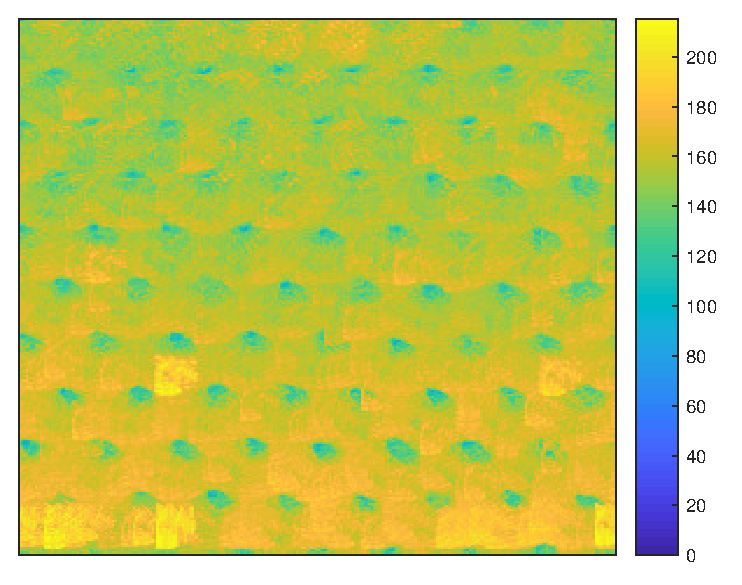
\includegraphics[width=.20\linewidth]{periodic_L1_20_superp_col.eps}} \hfill
  \subfloat{\includegraphics[width=.20\linewidth]{periodic_Linfinite_20_superp_col.eps}} \hfill
  \subfloat{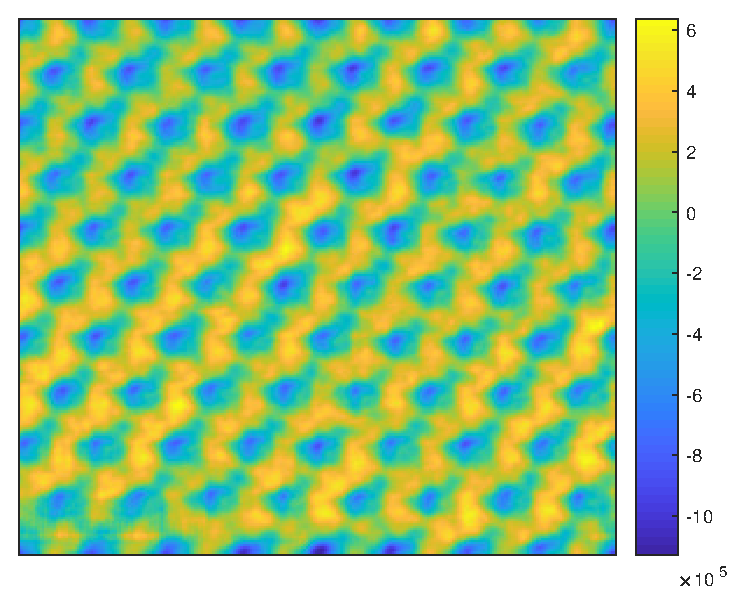
\includegraphics[width=.20\linewidth]{periodic_ps_20_superp_col.eps}} \hfill
  \subfloat{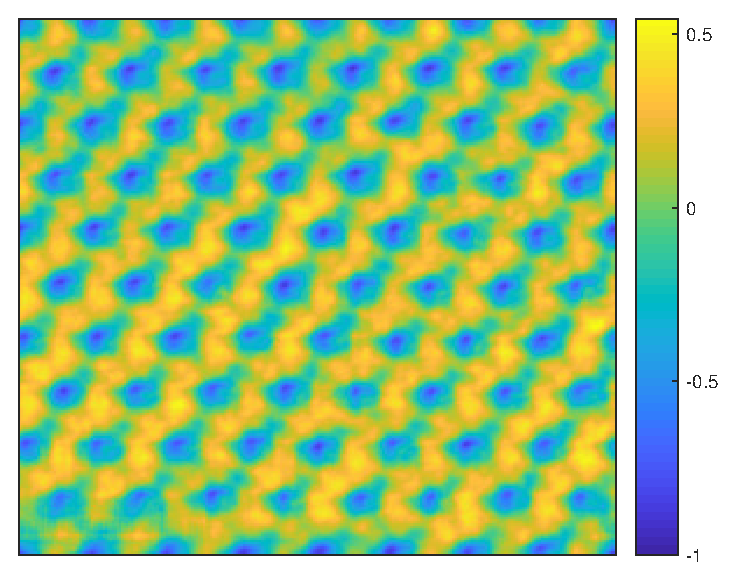
\includegraphics[width=.20\linewidth]{periodic_cos_20_superp_col.eps}} \hfill \\
  \subfloat{\includegraphics[width=.18\linewidth]{stochastic_L2_20_superp.png}} \hfill
  \subfloat{\includegraphics[width=.18\linewidth]{stochastic_L1_20_superp.png}} \hfill
  \subfloat{\includegraphics[width=.18\linewidth]{stochastic_Linfinite_20_superp.png}} \hfill
  \subfloat{\includegraphics[width=.18\linewidth]{stochastic_ps_20_superp.png}} \hfill
  \subfloat{\includegraphics[width=.18\linewidth]{stochastic_cos_20_superp.png}} \hfill \\
  \subfloat[\s2]{\includegraphics[width=.20\linewidth]{stochastic_L2_20_superp_col.eps}} \hfill
  \subfloat[\s1]{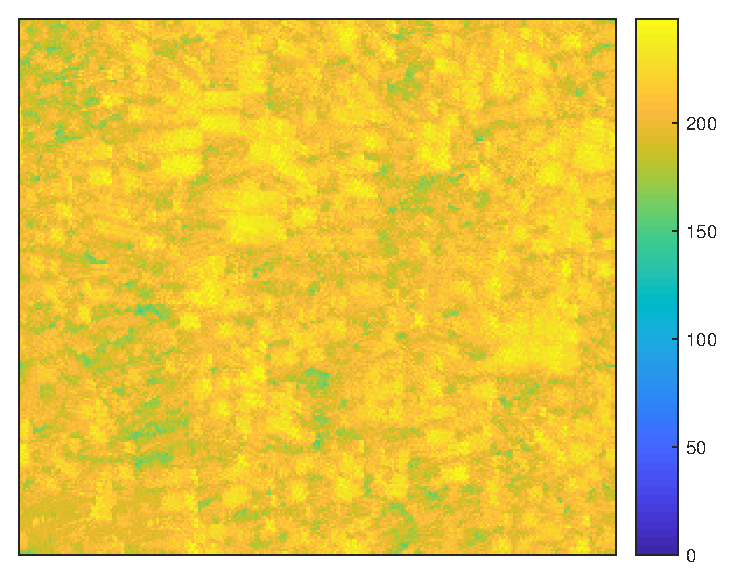
\includegraphics[width=.20\linewidth]{stochastic_L1_20_superp_col.eps}} \hfill
  \subfloat[\s{\infty}]{\includegraphics[width=.20\linewidth]{stochastic_Linfinite_20_superp_col.eps}} \hfill
  \subfloat[\sps]{\includegraphics[width=.20\linewidth]{stochastic_ps_20_superp_col.eps}} \hfill
  \subfloat[\scos]{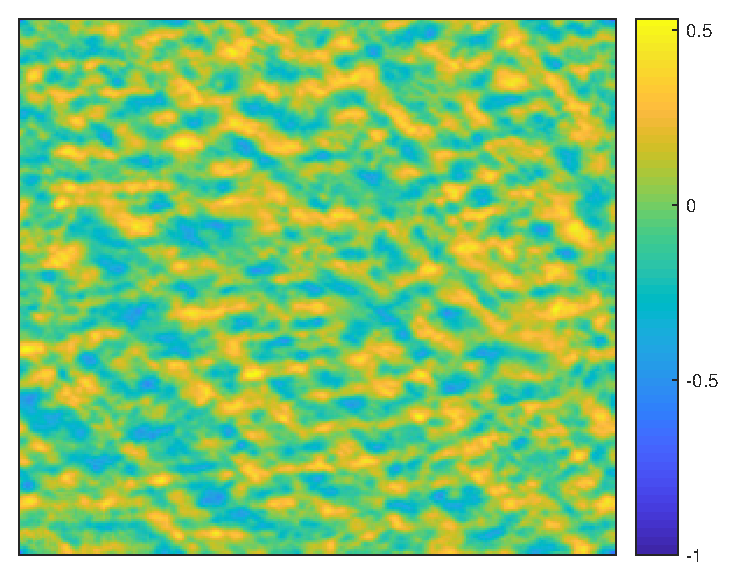
\includegraphics[width=.20\linewidth]{stochastic_cos_20_superp_col.eps}} \hfill
  \caption{We select the upper-left patch in texture (b) in Figure \ref{fig:textures}. Here the selected patch is $20 \times 20$. We then compare this patch to all the other patches of the textures using different patch similarity function. The first twenty best matches are shown in red for all the different similarity functions considered (first row). We then compute the map of the patch similarity function for the upper-left patch and the periodic texture (second row). We observe that every similarity function detects patches that are perceptually similar to the original patch. Note also that in every case the most similar patch is the original one. Note also that even if here the patches are really similar the similarity functions do not choose the same patches. This first test can be considered as a sanity check. On the last two rows we conduct the same study on the stochastic texture. It is really interesting to note that in this case the Euclidean distance do not yield innovation. Indeed only two patches and their shifted versions for small shifts are selected. \s1 \ yield a lot of different patches but a look at the similarity map indicate us that this similarity function is not likely to discriminate between patches. It can also be seen that the selected patches are not really similar to the original one. \s{\infty} \ gives better results. \sps \ selects patches which have very similar structure to the original one but are brighter. This effect is reduced in \scos \ which also yields satisfactory results.}
  \label{fig:sim_func1}
\end{figure}
\begin{figure}[H]
  \centering
  \subfloat{\includegraphics[width=.18\linewidth]{periodic_L2_05_superp.png}} \hfill
  \subfloat{\includegraphics[width=.18\linewidth]{periodic_L1_05_superp.png}} \hfill
  \subfloat{\includegraphics[width=.18\linewidth]{periodic_Linfinite_05_superp.png}} \hfill
  \subfloat{\includegraphics[width=.18\linewidth]{periodic_ps_05_superp.png}} \hfill
  \subfloat{\includegraphics[width=.18\linewidth]{periodic_cos_05_superp.png}} \hfill \\
  \subfloat{\includegraphics[width=.20\linewidth]{periodic_L2_05_superp_col.eps}} \hfill
  \subfloat{\includegraphics[width=.20\linewidth]{periodic_L1_05_superp_col.eps}} \hfill
  \subfloat{\includegraphics[width=.20\linewidth]{periodic_Linfinite_05_superp_col.eps}} \hfill
  \subfloat{\includegraphics[width=.20\linewidth]{periodic_ps_05_superp_col.eps}} \hfill
  \subfloat{\includegraphics[width=.20\linewidth]{periodic_cos_05_superp_col.eps}} \hfill \\
    \subfloat{\includegraphics[width=.18\linewidth]{contrast_L2_20_superp.png}} \hfill
  \subfloat{\includegraphics[width=.18\linewidth]{contrast_L1_20_superp.png}} \hfill
  \subfloat{\includegraphics[width=.18\linewidth]{contrast_Linfinite_20_superp.png}} \hfill
  \subfloat{\includegraphics[width=.18\linewidth]{contrast_ps_20_superp.png}} \hfill
  \subfloat{\includegraphics[width=.18\linewidth]{contrast_cos_20_superp.png}} \hfill \\
  \subfloat[\s2]{\includegraphics[width=.20\linewidth]{contrast_L2_20_superp_col.eps}} \hfill
  \subfloat[\s1]{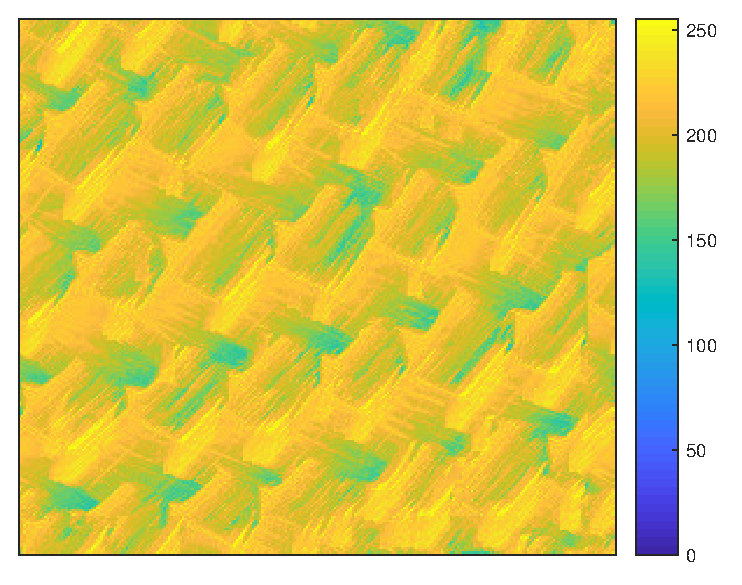
\includegraphics[width=.20\linewidth]{contrast_L1_20_superp_col.eps}} \hfill
  \subfloat[\s{\infty}]{\includegraphics[width=.20\linewidth]{contrast_Linfinite_20_superp_col.eps}} \hfill
  \subfloat[\sps]{\includegraphics[width=.20\linewidth]{contrast_ps_20_superp_col.eps}} \hfill
  \subfloat[\scos]{\includegraphics[width=.20\linewidth]{contrast_cos_20_superp_col.eps}} \hfill
  \caption{In this figure we reproduce the study conducted in the first row of Figure \ref{fig:sim_func1} but with a patch size of $5 \times 5$. In this case the patch corresponds to an uniform zone. Every similarity function gives good perceptual results. However \sps \ fails to yield different patches. This is due to the fact \sps \ is sensible to the illumination of the scene. Thus here it will choose the darkest spot. Note that it makes no sense to consider \sps if the image has not been normalized as it will simply select the brightest patch. An interesting phenomenon occurs looking at the second row, the \scos \ similarity measure seems to be far more discriminative than the others. This effect could have been guessed in Figure \ref{fig:sim_func1} but is far more visible here. The last two rows reproduce the same study with patch size equals to $20 \times 20$ and original image being the texture with illumination defect. Once again \sps \ produces bad results since it focuses on the illumination more than the structure.}
  \label{fig:sim_func2}
\end{figure}
\begin{figure}[H]
  \subfloat{\includegraphics[width=.18\linewidth]{stochastic_L2_15_superp.png}} \hfill
  \subfloat{\includegraphics[width=.18\linewidth]{stochastic_L1_15_superp.png}} \hfill
  \subfloat{\includegraphics[width=.18\linewidth]{stochastic_Linfinite_15_superp.png}} \hfill
  \subfloat{\includegraphics[width=.18\linewidth]{stochastic_ps_15_superp.png}} \hfill
  \subfloat{\includegraphics[width=.18\linewidth]{stochastic_cos_15_superp.png}} \hfill \\
  \subfloat{\includegraphics[width=.20\linewidth]{stochastic_L2_15_superp_col.eps}} \hfill
  \subfloat{\includegraphics[width=.20\linewidth]{stochastic_L1_15_superp_col.eps}} \hfill
  \subfloat{\includegraphics[width=.20\linewidth]{stochastic_Linfinite_15_superp_col.eps}} \hfill
  \subfloat{\includegraphics[width=.20\linewidth]{stochastic_ps_15_superp_col.eps}} \hfill
  \subfloat{\includegraphics[width=.20\linewidth]{stochastic_cos_15_superp_col.eps}} \hfill \\
  \subfloat[\s2]{\includegraphics[width=.18\linewidth]{stochastic_L2_15_ecdf.eps}} \hfill
  \subfloat[\s1]{\includegraphics[width=.18\linewidth]{stochastic_L1_15_ecdf.eps}} \hfill
  \subfloat[\s{infty}]{\includegraphics[width=.18\linewidth]{stochastic_Linfinite_15_ecdf.eps}} \hfill
  \subfloat[\sps]{\includegraphics[width=.18\linewidth]{stochastic_ps_15_ecdf.eps}} \hfill
  \subfloat[\scos]{\includegraphics[width=.18\linewidth]{stochastic_cos_15_ecdf.eps}} \hfill
  \caption{In this experiment we consider $15 \times 15$ patches and a stochastic texture. It is worth noticing that if \s1 \ and \sps \ yield poor results, \s2 , \s{\infty} and \scos \ give similar results. The positions identified using \scos \ and \s{\infty} \ are also identified by \s2 . Note also that the similarity maps vary a lot depending on the similarity function. However, the empirical c.d.f represented in the third row do not yield important information in order to identify the differences between these similarity functions.}
    \label{fig:sim_func3}
  \end{figure}
  \subparagraph{} We have seen in Figure \ref{fig:sim_func1} that the similarity functions gave satisfactory perceptual results. It is worth noticing, see \ref{fig:sim_func2} that the results highly depend on the size of the patch. We also show that the \s{\infty} \ and the \scos \ similarity function yield satisfactory perceptual results in Figure \ref{fig:sim_func3} even if \scos \ is not a distance. If the poor performance of the \sps \ similarity function was expected due to its sensibility to the illumination, the mild results of \s1 \ are more surprising. No satisfying explanation was found to explain this type of behaviour. In the next section we present the results obtained when applying these functions to random fields.
  \subsubsection{Similarity functions and p.d.f}
  In this section we will consider two cases:
  \begin{itemize}
  \item the white noise case where our spot in the \ADSN \ model will $\delta_0$,
  \item the full \ADSN \ model.
  \end{itemize}
  Our goal here is to confirm the results obtained in the previous section.
  We consider $\mathcal{P} = \llbracket 1,20 \rrbracket^2$ and $\Omega = \llbracket 1,512 \rrbracket^2$. We generate $N=1500$ \ADSN \ realizations.
  \begin{figure}[H]
    \centering
    \subfloat[white noise]{\includegraphics[width=0.24\linewidth]{white_noise.png}} \hfill
    \subfloat[mild \ADSN]{\includegraphics[width=0.24\linewidth]{mildADSN.png}} \hfill
    \subfloat[full \ADSN]{\includegraphics[width=0.24\linewidth]{fullADSN.png}} \\
    \subfloat{\includegraphics[width=0.24\linewidth]{white_noise_sample.png}} \hfill
    \subfloat{\includegraphics[width=0.24\linewidth]{mildADSN_sample.png}} \hfill
    \subfloat{\includegraphics[width=0.24\linewidth]{fullADSN_sample.png}} \hfill
    \caption{The spot is represented in the original domain $\Omega$. For example in the white noise the spot is only one white pixel in the upper-left corner. Same thing in the mild \ADSN \ which consists in a spot defined on $\llbracket 1,5 \rrbracket^2$ constant equals to one. The full \ADSN \ corresponds to a spot extracted from an image from the Simoncelli distaste. The spot is defined on $\llbracket 1,20\rrbracket^2$. On the second row we show one realization of the \ADSN \ model for each spot.}
    \label{fig:spot}    
  \end{figure}
    \begin{figure}[H]
    \centering
    \subfloat{\includegraphics[width=0.24\linewidth]{white_noise_offset_mat.png}} \hfill
    \subfloat{\includegraphics[width=0.24\linewidth]{mildADSN_offset_mat.png}} \hfill
    \subfloat{\includegraphics[width=0.24\linewidth]{fullADSN_offset_mat.png}} \\
    \subfloat[white noise]{\includegraphics[width=0.24\linewidth]{internal_l2_white_noise_20.eps}} \hfill
    \subfloat[mild \ADSN]{\includegraphics[width=0.24\linewidth]{internal_l2_mildADSN_20.eps}} \hfill
    \subfloat[full \ADSN]{\includegraphics[width=0.24\linewidth]{internal_l2_fullADSN_20.eps}} \hfill
    \caption{In this figure we show the offset correlation matrices for the different spots considered (first row). We also show the validity of Proposition REF. On each graph we represent the empirical c.d.f and the exact c.d.f computed with the Imhof integral.}
    \label{fig:l2}    
  \end{figure}
  \begin{figure}[H]
    \subfloat{\includegraphics[width=0.32\linewidth]{internal_ps_white_noise_20.eps}} \hfill
    \subfloat{\includegraphics[width=0.32\linewidth]{internal_ps_mildADSN_20.eps}} \hfill
    \subfloat{\includegraphics[width=0.32\linewidth]{internal_ps_fullADSN_20.eps}} \\
    \subfloat{\includegraphics[width=0.32\linewidth]{internal_cos_white_noise_20.eps}} \hfill
    \subfloat{\includegraphics[width=0.32\linewidth]{internal_cos_mildADSN_20.eps}} \hfill
    \subfloat{\includegraphics[width=0.32\linewidth]{internal_cos_fullADSN_20.eps}} \\
    \subfloat{\includegraphics[width=0.32\linewidth]{template_ps_white_noise_20.eps}} \hfill
    \subfloat{\includegraphics[width=0.32\linewidth]{template_ps_mildADSN_20.eps}} \hfill
    \subfloat{\includegraphics[width=0.32\linewidth]{template_ps_fullADSN_20.eps}} \\
    
    \subfloat[white noise]{\includegraphics[width=0.32\linewidth]{template_cos_white_noise_20.eps}} \hfill
    \subfloat[mild \ADSN]{\includegraphics[width=0.32\linewidth]{template_cos_mildADSN_20.eps}} \hfill
    \subfloat[full \ADSN]{\includegraphics[width=0.32\linewidth]{template_cos_fullADSN_20.eps}} \hfill
    \caption{In this figure we illustrate the convergence in law announced in Propositions REF. First row corresponds to \internalmatching \ and scalar product, i.e Proposition REF. Second row corresponds to \internalmatching \ and cosine, i.e Proposition REF. Third row corresponds to \templatematching \ and scalar product, i.e Proposition REF. Fourth row corresponds to \templatematching \ and cosine, i.e Proposition REF}
    \label{fig:tcl}
    \end{figure}

  \subsection{Continuous or discrete framework}
Implementation requires us to use the $\Omega = \mathbb{T}_M \times \mathbb{T}_N$ version of our results. So one could legitimately ask, why bother with continuous settings? Many answers can be formulated (interpolation purposes, infinite resolution...). We choose to highlight the fact that in the previous study only shifts were considered to compare patches. However it is a well-known fact that in order to compare to scenes homographies must be computed. Rotation and scaling do not react well with a discrete setting and therefore we must consider a continuous framework.\\
\comment{ Les calculs qui suivent sont des idées jetées sur \LaTeX ... pour
  comparer deux patches après transformation affine il est naturel de faire
  $\summ{x \in \Omega}{}{\vertt{\mathbb{1}_{x \in \mathcal{P}} I_1(x) -
      I_2(Ax)}^2} = \|f\|_2^2 + \|g(A\cdot)\|_2^2 + 2\summ{x \in
    \Omega}{}{f(x)g(Ax)}$ avec $f(x) = \mathbb{1}_{x \in \mathcal{P}}$ et
  $g(x) = I(x)$. On a envie de profiter d'un algorithme type \FFT \ pour
  calculer la somme dans le dernier terme. Pour cela introduisons l'opérateur
  $T$ qui va de $\hat{\mathbb{R}}$ dans $\hat{G_A}$.
  $\tilde{f}(A) := T(f)(A) = f(A(0))$. Ainsi
  \[\summ{x \in \Omega}{}{f(x)g(Ax)} = \int_{G_A} \tilde{f}(B)\mathbb{1}_{B\in
      \mathcal{T}} \tilde{g}(AB) \text{d}B\] où $\mathcal{T}$ est l'ensemble des
  translations. Si on arrive à définir une transformée de Fourier rapide sur ce
  groupe on peut, en un nombre d'itérations surlinéaire par rapport aux
  transformations affines. J'ai écrit les choses avec le groupe affine ici, on
  peut faire la même chose pour les homographies. On a une complexité en
  $\mathcal{O}(\vertt{G_A} \log(\vertt{G_A}))$ contre
  $\mathcal{O}(\vertt{G_A} \mathcal{P})$ en calculant les quantités
  ``naïvement'' = vrai gain lorsque l'on compare des gros patchs... Un autre
  intérêt est aussi de pouvoir bouger dans l'espace des homographies et/ou des
  transformations affines pour pouvoir identifier lesquelles présentent un
  intérêt (visualisation d'un tel espace ?)}
\\

%\end{document}
